\documentclass[12pt]{article}
 
\usepackage[margin=1in]{geometry}
\usepackage{amsmath,amsthm,amssymb}
\usepackage{commath}
\usepackage{graphicx}
\usepackage{float}
\usepackage{caption}
\usepackage{subcaption}
\usepackage{hyperref}
\usepackage{gensymb}
\usepackage{xparse,mathtools}
\usepackage{color,soul}
\usepackage{enumitem}
\usepackage{eufrak}
\usepackage{cleveref}
%\usepackage{datetime}

%%% --------- packages for glossary ------- %%%
\usepackage[acronym,nomain,nonumberlist]{glossaries}
\makeglossaries
%
\newacronym{LHS}{LHS}{left-hand side}
\newacronym{RHS}{RHS}{right-hand side}
\newacronym{CARA}{CARA}{Constant Absolute Risk-Aversion}
\newacronym{CRRA}{CRRA}{Constant Relative Risk-Aversion}
\newacronym{ADP}{ADP}{Approximate Dynamic Programming}
\newacronym{MDP}{MDP}{Markov Decision Process}
\newacronym{MO}{MO}{Market Order}
\newacronym{TOB}{TOB}{Trading Order Book}
\newacronym{LO}{LO}{limit order}

\usepackage[backend=bibtex,style=numeric]{biblatex}
% Select the bibliography file
\addbibresource{references.bib}

\ExplSyntaxOn

\NewDocumentCommand \vect { s o m }
 {
  \IfBooleanTF {#1}
   { \vectaux*{#3} }
   { \IfValueTF {#2} { \vectaux[#2]{#3} } { \vectaux{#3} } }
  ^T
 }

\DeclarePairedDelimiterX \vectaux [1] {\lbrack} {\rbrack}
 { \, \dbacc_vect:n { #1 } \, }

\cs_new_protected:Npn \dbacc_vect:n #1
 {
  \seq_set_split:Nnn \l_tmpa_seq { , } { #1 }
  \seq_use:Nn \l_tmpa_seq { \enspace }
 }
\ExplSyntaxOff
 
\newcommand{\N}{\mathbb{N}}
\newcommand{\R}{\mathbb{R}}
\newcommand{\Z}{\mathbb{Z}}
\newcommand{\Q}{\mathbb{Q}}

\newcommand{\myequation}{\begin{equation}}
\newcommand{\myendequation}{\end{equation}}
\let\[\myequation
\let\]\myendequation
 
\newenvironment{theorem}[2][Theorem]{\begin{trivlist}
\item[\hskip \labelsep {\bfseries #1}\hskip \labelsep {\bfseries #2.}]}{\end{trivlist}}
\newenvironment{lemma}[2][Lemma]{\begin{trivlist}
\item[\hskip \labelsep {\bfseries #1}\hskip \labelsep {\bfseries #2.}]}{\end{trivlist}}
\newenvironment{exercise}[2][Exercise]{\begin{trivlist}
\item[\hskip \labelsep {\bfseries #1}\hskip \labelsep {\bfseries #2.}]}{\end{trivlist}}
\newenvironment{problem}[2][Problem]{\begin{trivlist}
\item[\hskip \labelsep {\bfseries #1}\hskip \labelsep {\bfseries #2.}]}{\end{trivlist}}
\newenvironment{question}[2][Question]{\begin{trivlist}
\item[\hskip \labelsep {\bfseries #1}\hskip \labelsep {\bfseries #2.}]}{\end{trivlist}}
\newenvironment{corollary}[2][Corollary]{\begin{trivlist}
\item[\hskip \labelsep {\bfseries #1}\hskip \labelsep {\bfseries #2.}]}{\end{trivlist}}
\newenvironment{solution}
  {\renewcommand\qedsymbol{$\blacksquare$}\begin{proof}[Solution]}
  {\end{proof}}
 
\date{January 31, 2020}
 
\begin{document}
 
\title{Homework \#8}
\author{Junwu Zhang\\ 
CME 241: Reinforcement Learning for Finance \\}
%\date{}
\maketitle

\begin{problem}{1}
\text{ }\\
Work out (in LaTeX) the solution to the Linear Impact model we covered in class
\end{problem}
\begin{solution}
\text{ }\\
First of all, there are a number of terms that we should discuss and define here. 

The \gls{TOB} describes the relationship between volume, price per share, and the type of \gls{LO}. A typical \gls{TOB} is shown in \Cref{fig:TOB} below.

\begin{figure}[H]
\centering
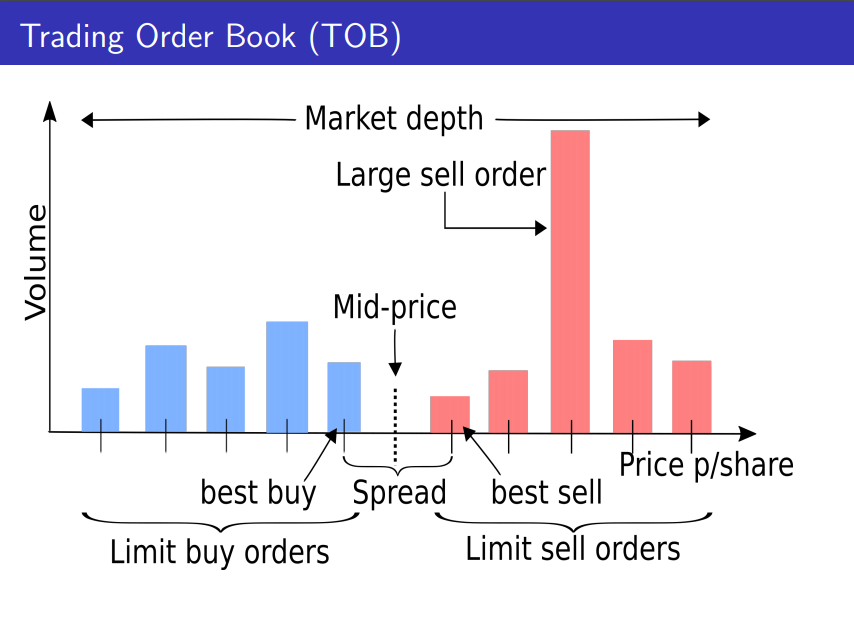
\includegraphics[width=0.8\textwidth]{TOB}
\caption{Typical \acrfull{TOB}}
\label{fig:TOB}
\end{figure}

A \gls{MO} alters the \gls{TOB}, and \textit{price impact} refers to how large-scale \gls{MO} moves the bid/ask/mid price of shares in the market. In this problem, we're looking at a linear price impact model, where the differences in \gls{MO} and prices are linearly related.

Second of all, we realize that we can formulate the entire optimal trade order execution problem as an \gls{MDP}. Our overall goal is to sell a large amount $N$ of shares, where trading happens in $T$ discrete time steps. Only \gls{MO}s are allowed, and we need to balance the speed of selling with the market price of the shares. More specifically, the \gls{MDP} can be constructed as following:

\textit{States} are ($t, P_t, R_t$) where $t$ represents the time step, $P_t$ denotes Bid Price at start of time step $t$, and $R_t = N - \sum_{i=1}^{t-1}N_i$ denotes shares remaining at start of time step $t$

\textit{Actions} is $N_t$ which denotes the number of shares sold in time step $t$

\textit{Reward} is $U(N_t \cdot Q_t)$

\textit{Price transition dynamics} is $P_{t+1} = f_t(P_t, N_t, \epsilon_t)$

Given all these elements, the objective is to find a policy $\pi^\ast(t, P_t, R_t)$ that maximizes:
\begin{equation}
\mathbb{E}[\sum_{t=1}^{T}\gamma^t \cdot U(N_t \cdot Q_t)]
\end{equation}
where $\gamma$ is the discount factor of the \gls{MDP}.

Once we have such \gls{MDP} problem definition, we can consider a model with linear price impact, where $N, N_t, P_t$ are all continuous. The price dynamics is given by:
\begin{equation}
P_{t+1} = P_t - \alpha N_t + \epsilon_t
\end{equation}
where $\alpha \in \mathbb{R}_{\leq0}$ and $\epsilon_t$ is i.i.d. with $\mathbb{E}[\epsilon_t \vert N_t, P_t] = 0$.

As a first step to solving this, we can denote the value function with policy $\pi$ as:
\begin{equation}
V^{\pi}\left(t, P_{t}, R_{t}\right)=\mathbb{E}_{\pi}\left[\sum_{i=t}^{T} N_{i}\left(P_{i}-\beta N_{i}\right) |\left(t, P_{t}, R_{t}\right)\right]
\end{equation}
Since optimal value function can be denoted as $V^{*}\left(t, P_{t}, R_{t}\right)=\max _{\pi} V^{\pi}\left(t, P_{t}, R_{t}\right)$, we can expand it to write:
\begin{equation}
V^{*}\left(t, P_{t}, R_{t}\right)=\max _{N_{t}}\left(N_{t}\left(P_{t}-\beta N_{t}\right)+\mathbb{E}\left[V^{*}\left(t+1, P_{t+1}, R_{t+1}\right)\right]\right)
\end{equation}
We can infer $V^{*}\left(T-1, P_{T-1}, R_{T-1}\right)$ as:
\begin{align}
& \max _{N_{T-1}}\left\{N_{T-1}\left(P_{T-1}-\beta N_{T-1}\right)+\mathbb{E}\left[R_{T}\left(P_{T}-\beta R_{T}\right)\right]\right\} \\
=& \max _{N_{T-1}}\left\{R_{T-1} P_{T-1}-\beta R_{T-1}^{2}+(\alpha-2 \beta)\left(N_{T-1}^{2}-N_{T-1} R_{T-1}\right)\right\}
\end{align}
Taking derivative and setting to zero, we have:
\begin{equation}
\label{eq:Nt-1}
	(\alpha-2 \beta)\left(N_{T-1}^{2}-N_{T-1} R_{T-1}\right) = 0 \rightarrow N^\ast_{T-1} = \frac{R_{T-1}}{2}
\end{equation}
Note that this is for the non-trivial case $\alpha < 2\beta$. 

Plug the result from \Cref{eq:Nt-1} in the expression for $V^*$, we have:
\begin{equation}
V^{*}\left(T-1, P_{T-1}, R_{T-1}\right)=R_{T-1} P_{T-1}-R_{T-1}^{2}\left(\frac{\alpha+2 \beta}{4}\right)
\end{equation}
Similarly, continuing backwards in time, we have:
\begin{equation}
\begin{array}{c}
N_{t}^{\star}=\frac{R_{t}}{T-t+1} \\
V^{*}\left(t, P_{t}, R_{t}\right)=R_{t} P_{t}-\frac{R_{t}^{2}}{2}\left(\frac{2 \beta+(T-t) \alpha}{T-t+1}\right)
\end{array}
\end{equation}
\end{solution}

\begin{problem}{2}
	\text{ }\\
Model a real-world Optimal Trade Order Execution problem as an MDP
\end{problem}

\begin{solution}
The \gls{MDP} can be modeled as:
\begin{itemize}[noitemsep]
	\item \textit{States}: ($t, P_{b_t}, P_{s_t}, R_{b_t}, R_{s_t}$) where $t$ represents the time step, $P_{b_t}$ denotes buy price at start of time step $t$, $P_{s_t}$ denotes sell price at start of time step $t$, $R_{b_t}$ denotes shares available to buy at start of time step $t$, and $R_{s_t}$ denotes shares available to sell at start of time step $t$
	\item \textit{Actions}: $N_t$ which denotes the number of shares sold in time step $t$
	\item \textit{Reward}: $U(N_t \cdot Q_t)$
	\item \textit{Price Impact}: In real-world scenario, price impact might be purely temporary and can be represented as:
	\begin{equation}
	P_{t+1}=P_{t} e^{Z_{t}}, X_{t+1}=\rho X_{t}+\eta_{t}, Q_{t}=P_{t}\left(1-\alpha N_{t}-\theta X_{t}\right)
	\end{equation}
\end{itemize}
\end{solution}


\end{document}